% -----------------------------------------------------------------------------
% Section: Interpretability
% Rewritten around two complementary views of model reliance.
% All figures referenced here already exist in figures/generated/ and
% report/figures/generated/; no figure generation is required.
% -----------------------------------------------------------------------------
\section{Interpretability}
\label{sec:interp}

\subsection{Question and Scope}
\label{subsec:interp_scope}

In this section we are looking at \emph{what does the trained AI-READI
forecasting model rely on?}
The answer is reported through two views:
The first view is \emph{output level reliance}: how much the 12 step forecast
changes when a modality is ablated.
The second view is \emph{state construction reliance}: how much each modality
contributes to the recurrent Mamba hidden state $h_t$ before the decoder turns
that state into a forecast.

All results in this section use the full held out AI-READI test split:
153{,}591 anchors sampled at a 15 minute stride across 381
participant/segment streams from 221 test participants.
The analysis is not restricted by insulin status metadata.

\subsection{Interpretability based on two directions}
\label{subsec:interp_two_views}

\paragraph{Interpretability view 1: output level reliance.}
Leave-one-modality-out (LOMO) ablation measures the mean absolute change in
the final 12step forecast when one modality is replaced by its population
mean.
This view is defined for all 11 modality groups because every group 
reaches the forecast decoder: glucose history, static clinical metadata,
site/cohort, time/calendar, data quality/missingness, heart rate/physiology,
medication metadata, sleep, wearable activity/exercise, stress, and the
meal-proxy diagnostic channel.
LOMO therefore answers a direct deployment question: if this information were
removed or made uninformative, how much would the forecast move?

\paragraph{Interpretability view 2: state construction reliance.}
The joint group norm measures how much a modality contributes to the
Mamba encoder hidden state $h_t$.
For each group $g$, per feature contribution vectors $u_f$ are summed first and
then normed, $\lVert\sum_{f\in g}u_f\rVert$.
Summing before taking the norm matters because many features are collinear:
heart-rate mean/min/max/std and multiple activity-stage indicators can point in
similar directions in representation space. The sum of individual norms would have double counted those shared directions.

The $h_t$ interpretability is available only for the 6 groups that pass through the
streaming encoder's grouped linear fusion into the recurrent state: glucose
history, heart rate/physiology, wearable activity/exercise, sleep, stress, and
data quality/missingness. 
Time/calendar and meal proxy feed the horizon decoder directly, while static
clinical metadata, medication metadata, and site/cohort modulate the decoder
through the static FiLM context.
Those groups are therefore interpreted through LOMO interpretability.


\subsection{View 1: Output-Level Reliance}
\label{subsec:interp_lomo}

Table~\ref{tab:interp_lomo_full} and Figure ~\ref{fig:interp_lomo_full} report
LOMO attribution on the full held-out test split.
The dominant output-level driver is \textbf{glucose history}: ablating it
changes the forecast by 5.87~mg/dL on average and accounts for 36.7\% of the
normalised output-level attribution.
This is the expected result for a residual-current CGM forecasting model:
recent glucose contains the strongest information about the next hour.

The next largest output-level group is \textbf{static clinical metadata}
(14.6\%, 2.33~mg/dL).
This does not mean that static variables cause short-term glucose movement;
it means the decoder uses phenotype and enrolment context to calibrate the
mapping from recent dynamics to future glucose.
\textbf{Site/cohort} (9.0\%) and \textbf{data quality/missingness} (8.4\%)
together account for 17.4\% of output-level reliance.
That is useful but also cautionary: part of the forecast depends on collection
structure, recruitment site, or missingness patterns rather than purely
physiological variation.

\textbf{Time/calendar} contributes 8.5\%, and \textbf{heart rate/physiology}
contributes 7.7\%.
Sleep, wearable activity/exercise, stress, and medication metadata have smaller
but nonzero output-level effects.
The \textbf{meal-proxy diagnostic channel} contributes 0.0\%, which is the
important negative control: under the available AI-READI representation, this
channel does not move the forecast and should not be interpreted as a meal
counterfactual mechanism.

\begin{table}[H]
  \centering
  \caption{%
    \textbf{Output-level modality reliance on the full held-out test split.}
    LOMO ablation measures the mean absolute change in the 12-step forecast
    when the named modality is replaced by its population mean.
    Fractions sum to 100\% across the 11 output-visible groups. %
  }
  \label{tab:interp_lomo_full}
  \small
  \begin{tabular}{lcc}
    \toprule
    Modality & Mean abs. change (mg/dL) & Fraction (\%) \\
    \midrule
    Glucose history               & 5.87 & 36.7 \\
    Static clinical               & 2.33 & 14.6 \\
    Site / cohort                 & 1.45 &  9.0 \\
    Time / calendar               & 1.35 &  8.5 \\
    Data quality / missingness    & 1.34 &  8.4 \\
    Heart rate / physiology       & 1.23 &  7.7 \\
    Medication metadata           & 0.70 &  4.4 \\
    Sleep                         & 0.65 &  4.0 \\
    Wearable activity / exercise  & 0.61 &  3.8 \\
    Stress                        & 0.48 &  3.0 \\
    Meal proxy (diagnostic only)  & 0.00 &  0.0 \\
    \bottomrule
  \end{tabular}
\end{table}

\begin{figure}[H]
  \centering
  
\includegraphics[width=0.86\linewidth]{generated/fig_interpret_lomo_full_attribution_v2.pdf}
  \caption{%
    \textbf{Output-level LOMO attribution on the full held-out test split
    ($n=153{,}591$ anchors).}
    Bars show the mean absolute forecast change after replacing each modality
    by its population mean.
    Glucose history is the largest output-moving input group, followed by
    static clinical context, site/cohort, time/calendar, data quality, and
    heart-rate/physiology.
    The meal-proxy diagnostic channel has no measurable output-level effect. %
  }
  \label{fig:interp_lomo_full}
\end{figure}

Fig.~\ref{fig:interp_lomo_full} places physiological and non-physiological
inputs on the same scale.
The important interpretation is not only that glucose dominates, but also that
site/cohort and data-quality signals remain visible in the output.
Those groups may improve forecast accuracy, but they also indicate possible
reliance on recruitment and measurement structure.



\subsection{View 2: State-Construction Reliance}
\label{subsec:interp_h_t}

The $h_t$ view changes the interpretation.
Among the 6 groups that actually enter the streaming recurrent state, glucose
history is still important but no longer overwhelming.
The rigorous joint-group norm assigns 21.9\% of state-construction reliance to
\textbf{glucose history}, 19.4\% to \textbf{heart rate/physiology}, and 18.9\%
to \textbf{data quality/missingness}.
\textbf{Sleep} (14.9\%), \textbf{wearable activity/exercise} (13.4\%), and
\textbf{stress} (11.6\%) make up the remainder.

This means the recurrent state is not just a compressed glucose trace.
It also stores information about physiology, missingness, sleep/activity
context, and stress-related channels.
The decoder then decides how much of that internal state should affect the
final forecast.
That distinction explains why wearable activity and sleep can matter much more
for $h_t$ construction than for output-level LOMO: they help build the internal
state, but the final forecast is still dominated by recent glucose and static
calibration.

\begin{table}[H]
  \centering
  \caption{%
    \textbf{State-construction reliance in the recurrent hidden state $h_t$.}
    Rigorous attribution uses $\lVert\sum_{f \in g}u_f\rVert$, summing each
    group's contribution vectors before taking the norm.
    Post-hoc sum uses $\sum_{f \in g}\lVert u_f\rVert$ and is shown only to
    illustrate collinearity-driven overcounting.
    The LOMO output column renormalises output-level reliance over the same
    6 $h_t$-reachable groups. %
  }
  \label{tab:interp_h_t_rigorous}
  \small
  \setlength{\tabcolsep}{4pt}
  \begin{tabular}{lcccc}
    \toprule
    Modality ($h_t$-reachable) & Rigorous (\%) & Post-hoc sum (\%) & Ratio & LOMO output, renorm. (\%) \\
    \midrule
    Glucose history               & 21.9 &  9.7 & 0.44 & 57.8 \\
    Heart rate / physiology       & 19.4 & 24.2 & 1.25 & 12.1 \\
    Data quality / missingness    & 18.9 & 22.9 & 1.21 & 13.2 \\
    Sleep                         & 14.9 & 10.1 & 0.68 &  6.4 \\
    Wearable activity / exercise  & 13.4 & 20.5 & 1.54 &  6.0 \\
    Stress                        & 11.6 & 12.5 & 1.08 &  4.7 \\
    \bottomrule
  \end{tabular}
\end{table}

\begin{figure}[H]
  \centering
  
\includegraphics[width=0.86\linewidth]{generated/fig_interpret_importance_grouped_aireadi_v2.pdf}
  \caption{%
    \textbf{Grouped state-construction importance (AI-READI v2).}
    Bars show each $h_t$-reachable group's rigorous joint-group-norm share.
    Glucose, heart-rate/physiology, and data-quality/missingness carry similar
    state-construction weight, while sleep, activity, and stress provide
    additional context that is less visible in output-level ablation. %
  }
  \label{fig:interp_h_t_rigorous}
\end{figure}

The grouped-importance view shows that the recurrent state is distributed
rather than glucose-only.

This second view is the representation-facing counterpart to the LOMO figures:
it asks what information the encoder stores, not what immediately moves the
decoder output.
The difference between these views is scientifically important because wearable,
sleep, stress, and data-quality channels can shape the internal state even when
the final forecast remains most sensitive to recent glucose.


  \label{fig:interp_global_ht_v2}
\end{figure}

\subsection{Reconciling the Two Views}
\label{subsec:interp_reconcile}

Fig.~\ref{fig:interp_state_vs_output} places the two reliance views next to
each other.
The central finding is an asymmetry between \emph{representation} and
\emph{forecast movement}.
Glucose history dominates forecast movement, but the hidden state distributes
its capacity more evenly across physiological, behavioral, and data-quality
channels.
Wearable activity/exercise and sleep are the clearest examples: their
state-construction shares are roughly 13--15\%, but their output-level LOMO
shares are only about 4\%.
The model appears to encode these channels as contextual state information;
the decoder only lets a smaller part of that context move the final forecast.

\begin{figure}[H]
  \centering
  
\includegraphics[width=0.92\linewidth]{generated/fig_interp_state_vs_output_v2.pdf}
  \caption{%
    \textbf{State-construction reliance versus output-level reliance.}
    The same $h_t$-reachable groups are compared under the rigorous state norm
    and output-level LOMO attribution.
    The figure shows that representation importance and forecast sensitivity
    are not interchangeable: glucose drives the forecast most strongly, while
    wearable and sleep channels contribute more to the internal state than to
    immediate output movement. %
  }
  \label{fig:interp_state_vs_output}
\end{figure}

The post-hoc comparison in Fig.~\ref{fig:interp_raw_vs_normalized} explains why
the rigorous group norm is necessary.
For collinear groups such as heart-rate/physiology and wearable
activity/exercise, summing individual feature norms after the fact inflates the
apparent group share.
The rigorous method avoids this by summing contribution vectors before taking
the norm.
This is why glucose history's post-hoc share looks artificially small: its
absolute contribution is not reduced, but the denominator is inflated by other
collinear groups.

\begin{figure}[H]
  \centering
  
\includegraphics[width=0.88\linewidth]{generated/fig_interp_raw_vs_normalized_v2.pdf}
  \caption{%
    \textbf{Why the rigorous joint-group norm is used.}
    Ratios above 1 indicate groups whose post-hoc sum-of-norms attribution is
    inflated by collinearity.
    The rigorous group norm is the appropriate state-construction measure
    because it counts shared directions once rather than once per correlated
    feature. %
  }
  \label{fig:interp_raw_vs_normalized}
\end{figure}

% ============================================================
\subsection{Static Clinical Interpretation}
\label{subsec:interp_static_clinical}
% ============================================================

Static covariates describe participant-level characteristics that remain fixed
over the monitored time series, including glycaemic status, baseline clinical
measurements, demographics, medication metadata, and clinical site. Their role
differs from that of streaming variables. Historical glucose and wearable
measurements describe the participant's current state, whereas static variables
provide a participant-specific context for interpreting those measurements.

The static analysis addresses three separate questions:

\begin{enumerate}
    \item How much does each static domain or feature change the final forecast?
    \item Does this dependence improve held-out predictive performance?
    \item Through which architectural pathway does the static information affect
    the model?
\end{enumerate}

These questions are evaluated separately because a feature can substantially
change the forecast without improving its accuracy.

% ------------------------------------------------------------
\subsubsection{Output Sensitivity and Predictive Usefulness}
\label{subsec:interp_static_output}
% ------------------------------------------------------------

For a static feature or domain $g$, output sensitivity is measured using
leave-one-group-out reference ablation. Let
$\widehat{\mathbf{y}}_i$ denote the original forecast at anchor $i$ and
$\widehat{\mathbf{y}}_i^{(-g)}$ the forecast obtained after replacing $g$ by
its training-derived reference representation. The raw sensitivity is

\begin{equation}
A_g =
\frac{1}{NH}
\sum_{i=1}^{N}
\sum_{h=1}^{H}
\left|
\widehat{y}_{i,h}
-
\widehat{y}_{i,h}^{(-g)}
\right|,
\label{eq:static_lomo_sensitivity}
\end{equation}

where $A_g$ is expressed in mg/dL. A large value indicates that the trained
model changes its forecasts when that information is removed. It does not by
itself indicate that the feature improves accuracy.

Predictive usefulness is evaluated using

\begin{equation}
\Delta\mathrm{MAE}_g
=
\mathrm{MAE}_{-g}
-
\mathrm{MAE}_{\mathrm{full}}.
\label{eq:static_predictive_usefulness}
\end{equation}

A positive value means that removing the feature worsens held-out MAE and that
the feature is predictively useful in the frozen model. A value close to zero
indicates limited incremental predictive value, whereas a negative value means
that the ablated model performs better. Negative frozen-model ablation results
do not automatically justify removing a feature, since replacing a feature
after training is not equivalent to retraining the architecture without it.

At the domain level, glycaemic-severity information produces the largest
forecast change, followed by demographic information. Medication metadata,
site/cohort, metabolic laboratory measurements, cardiovascular variables, and
anthropometric measurements have smaller effects. Domain-level values should be
interpreted cautiously because the domains contain different numbers of
features and different degrees of internal correlation.

\begin{figure}[t]
    \centering
    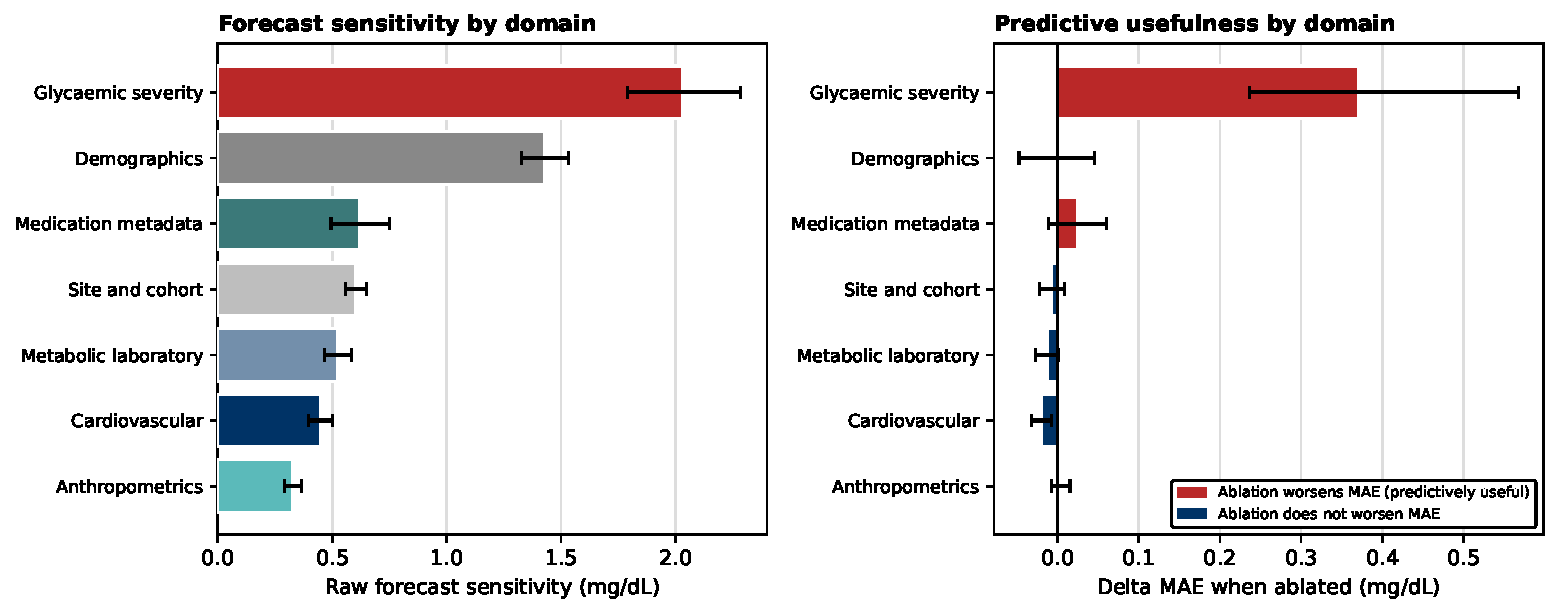
\includegraphics[width=\linewidth]
    {figures/generated/fig_interp_static_domains_v2.pdf}
    \caption{
    \textbf{Static-domain output sensitivity.}
    Bars show the mean absolute change in the 12-step forecast after replacing
    one static domain by its training-derived reference representation. Error
    bars show participant-clustered bootstrap confidence intervals. Glycaemic
    severity and demographics produce the largest output changes. The values
    measure model reliance in mg/dL and do not represent causal clinical
    effects or accuracy improvements.
    }
    \label{fig:interp_static_domains}
\end{figure}

The feature-level comparison provides a more precise interpretation of the
aggregated static-clinical result. Study group, baseline HbA1c, and baseline
serum glucose are both influential and predictively useful: their removal
changes the forecast and increases held-out MAE. These variables therefore
provide participant-level information that is not fully recoverable from the
recent CGM trajectory alone.

Study group is the strongest individual static feature. This variable
summarizes broad differences in glycaemic phenotype, including normoglycaemia,
prediabetes, non-insulin-treated diabetes, and insulin-treated diabetes.
However, its attribution should not be interpreted as an isolated clinical
effect because it is correlated with HbA1c, glucose variability, medication
status, and other participant characteristics.

HbA1c is the most influential continuous clinical measurement. Its positive
predictive usefulness indicates that long-term glycaemic control helps the
model adapt near-term forecasts across participants. Baseline serum glucose
provides an additional, smaller participant-level glycaemic prior.

In contrast, several demographic variables substantially change the forecast
but provide little or uncertain improvement in MAE. Marital status is a
particularly clear example of high sensitivity with limited predictive
usefulness. Race, ethnicity, sex, and site variables also require caution.
Their influence may reflect population structure, socioeconomic or behavioural
proxies, clinical-site differences, missingness patterns, or shortcut learning
rather than robust physiological information.

\begin{figure}[t]
    \centering
    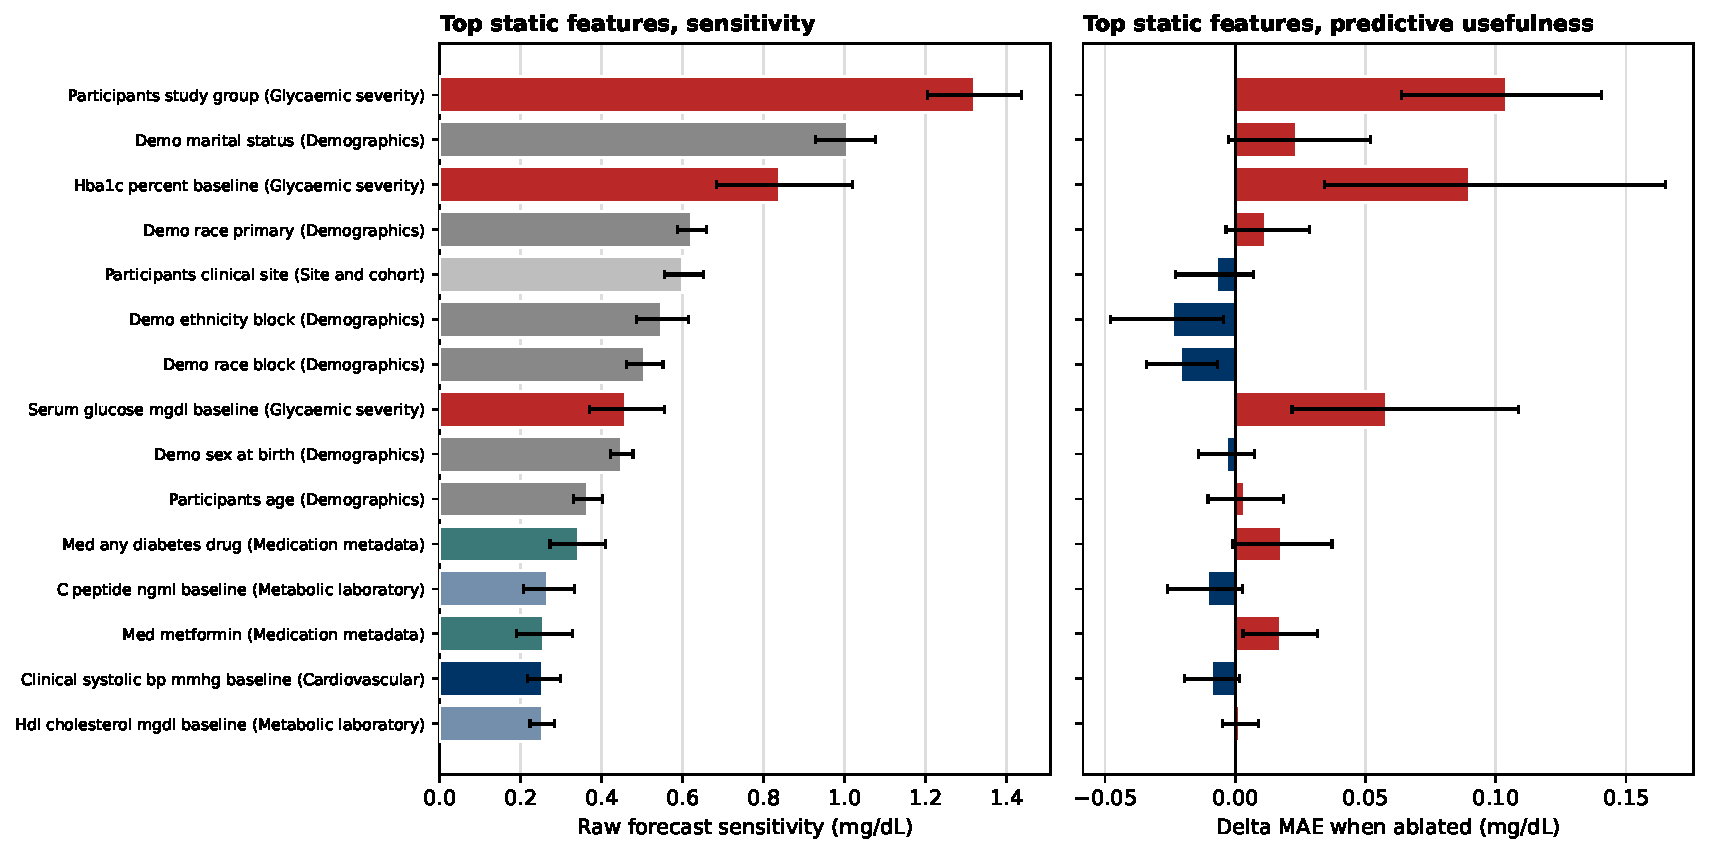
\includegraphics[width=\linewidth]
    {figures/generated/fig_interp_static_features_v2.pdf}
    \caption{
    \textbf{Static-feature reliance and predictive usefulness.}
    Left: raw mean absolute forecast change after reference ablation of each
    feature or categorical feature block. Right:
    $\Delta\mathrm{MAE}=\mathrm{MAE}_{-g}-\mathrm{MAE}_{\mathrm{full}}$.
    Positive values on the right indicate that removing the feature worsens
    prediction and that the feature is useful in the frozen model. Features may
    therefore be strongly used without providing a corresponding accuracy
    benefit. Categorical variables represented by multiple one-hot columns are
    ablated jointly as conceptual blocks.
    }
    \label{fig:interp_static_features}
\end{figure}

The feature-level results can be summarized into four categories:

\begin{itemize}
    \item \textbf{Strongly used and useful:}
    study group, HbA1c, and baseline serum glucose.
    
    \item \textbf{Strongly used but weakly useful:}
    marital status and selected demographic variables.
    
    \item \textbf{Neutral or potentially harmful under frozen-model ablation:}
    selected race/ethnicity blocks, clinical site, C-peptide, and other
    variables whose confidence intervals include or fall below
    $\Delta\mathrm{MAE}=0$.
    
    \item \textbf{Secondary static variables:}
    anthropometric, cardiovascular, and lipid measurements with relatively
    small forecast effects.
\end{itemize}

These findings motivate retrained ablation experiments rather than immediate
feature deletion. Protected demographic and site variables should additionally
be evaluated using conditional permutation or matched ablation within study
group, HbA1c range, and clinical site.

% ------------------------------------------------------------
\subsubsection{Static Conditioning Pathways}
\label{subsec:interp_static_pathways}
% ------------------------------------------------------------

Output-level ablation establishes that static information changes the
forecast, but it does not identify where that dependence enters the
architecture. Static covariates influence the model through several pathways.
The static representation initializes the participant-specific recurrent state,

\begin{equation}
h_0 = \psi(e_S),
\label{eq:static_h0}
\end{equation}

and conditions the historical representation using feature-wise linear
modulation,

\begin{equation}
u_t^{\mathrm{cond}}
=
\gamma(e_S)\odot u_t+\beta(e_S),
\label{eq:static_film}
\end{equation}

where $\gamma(e_S)$ multiplicatively rescales the dynamic representation and
$\beta(e_S)$ applies an additive shift.

For each static domain, the pathway analysis replaces that domain by its
training-derived reference representation and measures the resulting change in
$h_0$, $\gamma$, $\beta$, and the final forecast. The first three quantities
are representation-space $L_2$ norms, whereas output sensitivity is expressed
in mg/dL. Their absolute magnitudes are therefore not directly comparable
between panels.

\begin{figure}[t]
    \centering
    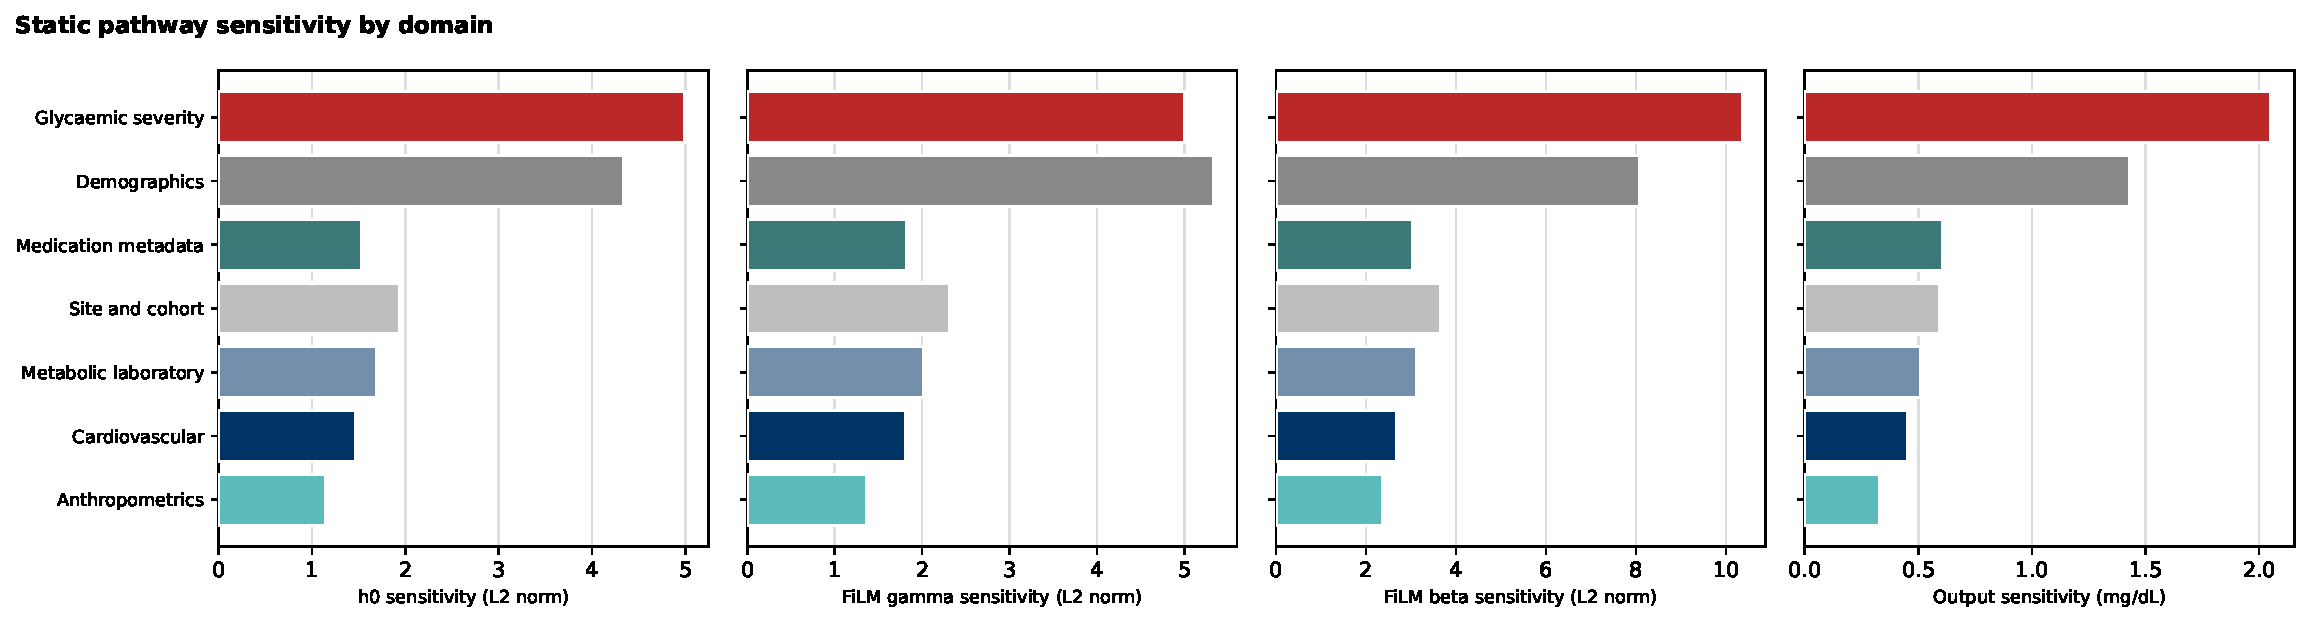
\includegraphics[width=\linewidth]
    {figures/generated/fig_interp_static_pathways_v2.pdf}
    \caption{
    \textbf{Static-domain sensitivity across model-conditioning pathways.}
    Each panel measures the change produced by replacing one static domain with
    its training-derived reference representation. From left to right, the
    panels show sensitivity of the participant-specific initial state $h_0$,
    the FiLM multiplicative scale $\gamma(S)$, the FiLM additive shift
    $\beta(S)$, and the final forecast output. Glycaemic-severity and
    demographic variables have the largest influence across the
    static-conditioning pathways, indicating that they affect both participant
    initialization and the processing of subsequent dynamic inputs. The first
    three panels report representation-space $L_2$ norms, whereas the final
    panel reports mean absolute forecast change in mg/dL. Magnitudes should
    therefore be compared across domains within each panel, not directly
    between panels. These quantities measure model sensitivity and do not
    represent causal effects.
    }
    \label{fig:interp_static_pathways}
\end{figure}

The pathway ranking is consistent with the output-level analysis. Glycaemic
severity has the largest effect on the initial state, the additive FiLM shift,
and the final output. This suggests that glycaemic phenotype establishes a
participant-specific metabolic baseline that persists throughout the streaming
forecast.

Demographic information also strongly affects all three static-conditioning
pathways and is particularly influential in the FiLM scaling pathway. This
means that demographic variables can change not only the initial participant
representation but also how subsequent dynamic glucose and wearable signals are
scaled by the model. This result is important for model auditing because it
creates a possible mechanism through which protected attributes or correlated
population structure can influence every later streaming update.

Medication, site/cohort, laboratory, cardiovascular, and anthropometric domains
have smaller but non-zero pathway sensitivities. Their effects are more
consistent with secondary participant-level adjustments than with dominant
short-horizon forecast drivers.

% ------------------------------------------------------------
\subsubsection{Sensitivity Across Clinical Values and Forecast Horizons}
\label{subsec:interp_static_curves}
% ------------------------------------------------------------

For selected continuous static variables, the original value is replaced by
training-distribution quantiles while all other inputs are held fixed. For
feature $j$, quantile $q$, and horizon $h$, the magnitude of the resulting
forecast change is

\begin{equation}
M_{j,q,h}
=
\frac{1}{N}
\sum_{i=1}^{N}
\left|
\widehat{y}_{i,h}
-
\widehat{y}_{i,h}
\left(S_{i,j}=Q_{j,q}\right)
\right|.
\label{eq:static_quantile_sensitivity}
\end{equation}

This experiment evaluates model sensitivity across the observed training
distribution. It is not a clinical intervention and should not be interpreted
as the effect of changing HbA1c, BMI, age, or another participant
characteristic.

\begin{figure}[t]
    \centering
    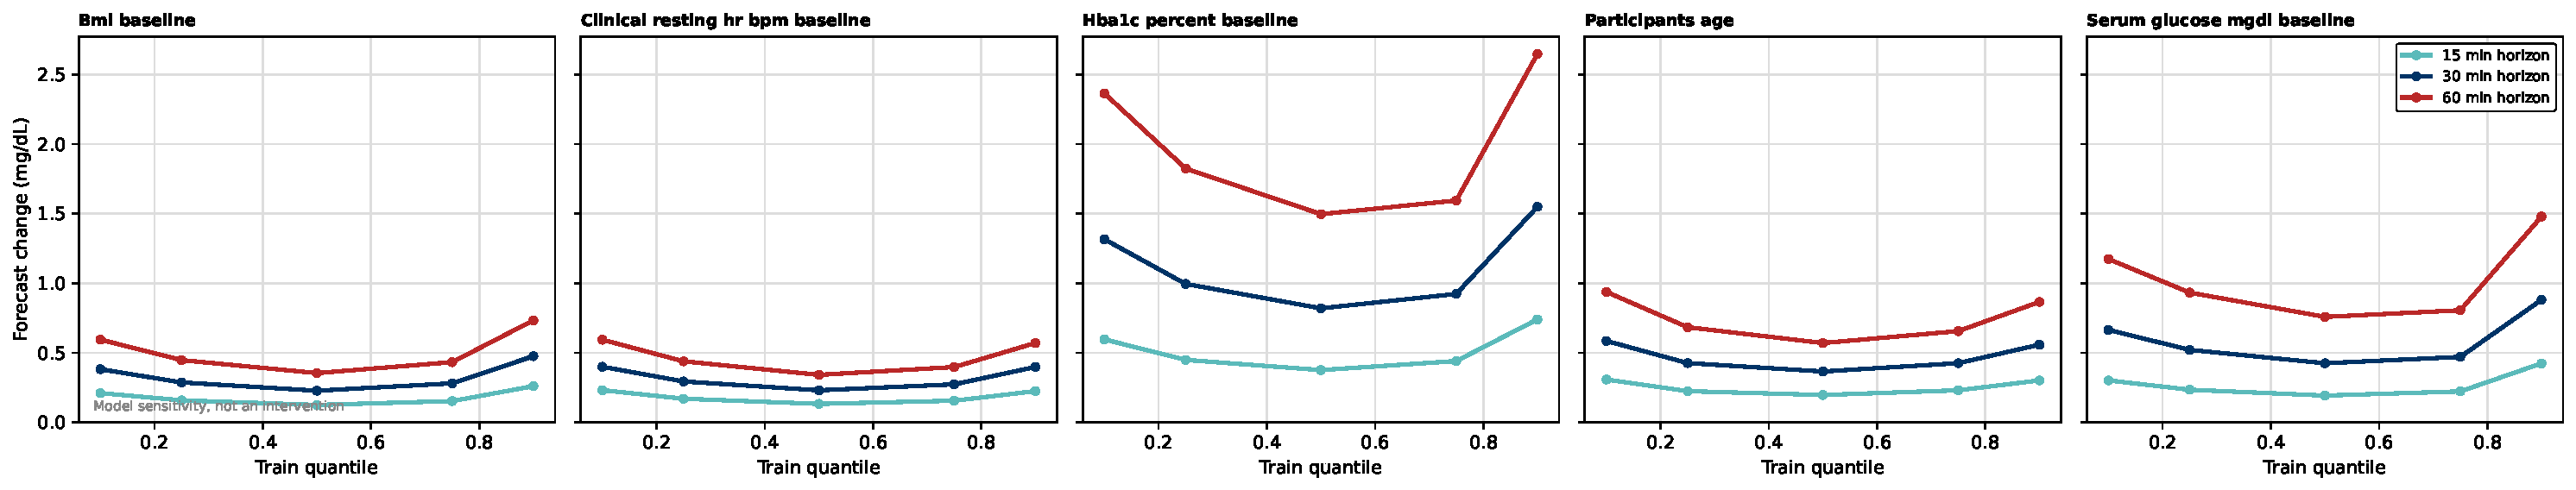
\includegraphics[width=\linewidth]
    {figures/generated/fig_interp_static_sensitivity_curves_v2.pdf}
    \caption{
    \textbf{Static-feature sensitivity across training-distribution quantiles.}
    Selected continuous variables are replaced by their training-split
    quantiles, and the resulting mean absolute forecast change is shown at
    15-, 30-, and 60-minute horizons. Static influence generally increases with
    forecast horizon. HbA1c has the largest continuous sensitivity, followed by
    baseline serum glucose, whereas BMI, age, and resting heart rate produce
    smaller changes. Because the plotted quantity is absolute, the curves show
    magnitude but not whether a given value raises or lowers the forecast.
    These are model-sensitivity analyses, not interventions.
    }
    \label{fig:interp_static_sensitivity}
\end{figure}

The horizon dependence is consistent across the selected variables:
participant-level static information has limited influence at the shortest
horizons, where the latest CGM reading dominates, but becomes more influential
towards 60 minutes as the decoder relies more heavily on participant-specific
priors.

HbA1c produces the largest sensitivity across the tested horizons, reinforcing
its role as the most important continuous static clinical variable. Baseline
serum glucose also modifies the longer-horizon prediction, while BMI, age, and
resting heart rate have smaller effects. The approximately U-shaped magnitude
curves indicate that replacing a participant's value with an extreme
population quantile changes the forecast more than replacing it with a typical
value. Since absolute changes are plotted, this pattern does not establish
whether low or high values raise the forecast.

% ------------------------------------------------------------
\subsubsection{Interpretation and Clinical Cautions}
\label{subsec:interp_static_cautions}
% ------------------------------------------------------------

The static analysis supports three principal conclusions.

First, static clinical information is not a single homogeneous input block.
Most of its useful predictive contribution is concentrated in variables that
describe glycaemic phenotype, particularly study group, HbA1c, and baseline
serum glucose.

Second, glycaemic-severity variables influence several architectural pathways.
They affect participant initialization, FiLM conditioning, and the final
forecast. Their high output reliance is therefore not solely an output-layer
artefact.

Third, the strong sensitivity to demographic and site variables requires
additional auditing. High reliance does not guarantee robust predictive value,
and a variable that improves performance on the current held-out split may
still reduce fairness or transportability under a new population, site, or
data-collection protocol.

The results therefore motivate three follow-up analyses:

\begin{enumerate}
    \item retraining the model without weak or potentially harmful static
    features;
    \item conditional demographic and site ablations within matched clinical
    strata;
    \item subgroup calibration and error analysis across protected and clinical
    categories.
\end{enumerate}

Overall, the model uses static clinical information primarily to construct a
participant-specific glycaemic prior. This improves forecasting when the static
variable captures stable metabolic phenotype, but it also creates a pathway
through which demographic, site, and measurement-process structure can
influence the prediction.


\subsection{Interpreting Non-Glucose Reliance}
\label{subsec:interp_non_glucose}

The non-glucose reliance results are important because they separate useful
context from potential shortcuts.
Heart-rate/physiology, sleep, activity, stress, and data-quality channels all
help construct $h_t$.
That does not imply that each channel has a large independent causal effect on
next-hour glucose.
It means the model has learned to encode these channels as part of the current
state from which the forecast is decoded.

The wearable subgroup figure shows that the activity/sleep block is not a
single opaque signal.
The model distributes state reliance across activity intensity, sleep-stage,
and data-quality-related channels.
This supports the interpretation that the recurrent state stores behavioral
context, not just CGM history.
At the same time, the data-quality detail figure shows why this must be read
cautiously: missingness and quality indicators are useful to the model but may
reflect device wear, site workflow, or participant adherence rather than
physiology.

\begin{figure}[H]
  \centering
  
\includegraphics[width=0.95\linewidth]{generated/fig_interp_wearable_subgroups_v2.pdf}
  \caption{%
    \textbf{Wearable and data-quality subgroup contributions to $h_t$.}
    The recurrent state uses several behavioral and quality-related channels
    rather than a single activity proxy.
    This is evidence of contextual state encoding, not by itself evidence of a
    causal activity effect. %
  }
  \label{fig:interp_wearable_subgroups}
\end{figure}

\begin{figure}[H]
  \centering
  
\includegraphics[width=0.95\linewidth]{generated/fig_interp_data_quality_detail_v2.pdf}
  \caption{%
    \textbf{Data-quality and missingness detail.}
    Data-quality channels contribute to both state construction and output
    behavior.
    This improves prediction but also flags a deployment concern: the model may
    partially exploit measurement process, device coverage, or site-specific
    missingness structure. %
  }
  \label{fig:interp_data_quality_detail}
\end{figure}

\subsection{Hidden-State Sanity Checks}
\label{subsec:interp_hidden_state_checks}

The probe figures ask whether $h_t$ contains clinically meaningful state
information after the streaming encoder has fused the input groups.
The regression probes show that the hidden state carries strong information
about current glucose and short-term glucose dynamics.
The classification probes show separability for categorical state targets, but
these should be interpreted as representation diagnostics rather than as
standalone clinical classifiers.
The PCA view provides a simple geometric check: the first principal component
of $h_t$ tracks current glucose strongly (correlation 0.821), indicating that
current glycemic state is a dominant axis of the learned representation.

\begin{figure}[H]
  \centering
  
\includegraphics[width=0.95\linewidth]{generated/fig_ht_probe_regression_v2.pdf}
  \caption{%
    \textbf{Hidden-state regression probes.}
    Probe performance indicates that $h_t$ contains recoverable information
    about current glucose and short-term dynamic state, consistent with the
    reliance results above. %
  }
  \label{fig:interp_probe_regression}
\end{figure}

\begin{figure}[H]
  \centering
  
\includegraphics[width=0.95\linewidth]{generated/fig_ht_probe_classification_v2.pdf}
  \caption{%
    \textbf{Hidden-state classification probes.}
    Classification probes test whether categorical state information is encoded
    in $h_t$.
    These are representation checks, not deployment classifiers. %
  }
  \label{fig:interp_probe_classification}
\end{figure}

\begin{figure}[H]
  \centering
  
\includegraphics[width=0.78\linewidth]{generated/fig_ht_pca_current_glucose_v2.pdf}
  \caption{%
    \textbf{PCA projection of $h_t$ colored by current glucose.}
    The first principal component is strongly aligned with current glucose
    (correlation 0.821; PC1 variance 28.0\%, PC2 variance 16.6\%), confirming
    that glycemic state is a major organizing direction of the hidden state. %
  }
  \label{fig:interp_pca}
\end{figure}

\subsection{Interpretation and Limitations}
\label{subsec:interp_limitations}

The two-view analysis supports four conclusions.
First, the forecast is primarily driven by glucose history, as it should be for
short-horizon CGM prediction.
Second, the hidden state is more distributed than the output attribution: it
stores physiology, activity/sleep context, stress, and data-quality structure
in addition to glucose history.
Third, Data-quality and site/cohort variables improve prediction on the current held-out cohort, but their contribution may reflect sensor availability, collection procedures, or population differences rather than direct physiological information. Their robustness should therefore be evaluated under unseen sites, devices, and missingness patterns before deployment.
Fourth, the meal-proxy diagnostic channel has no measurable output-level
influence in this run, so the AI-READI model should not be described as having
learned an interpretable meal counterfactual.

The main limitation is that these are reliance measures, not causal effect
estimates.
LOMO ablation asks how the trained model's output changes under a replacement
operation; it does not identify what would happen biologically if a modality
changed in the real world.
The $h_t$ joint-group norm asks how the encoder constructs its internal state;
it does not say which input would independently change the forecast under an
intervention.
Together, the two views give a defensible account of model reliance: what moves
the output, what builds the hidden state, and where predictive performance may
be borrowing from non-physiological structure.
